\documentclass{article}


% This is now the recommended way for checking for PDFLaTeX:
\usepackage{ifpdf}

% Use utf-8 encoding for foreign characters
\usepackage[utf8]{inputenc}

% Swedish grammar
\usepackage[swedish]{babel}

% Space between paragraphs instead of indentation.
\usepackage{parskip}

\ifpdf
\usepackage[pdftex]{graphicx}
\else
\usepackage{graphicx}
\fi

\ifpdf
\DeclareGraphicsExtensions{.pdf, .jpg, .tif, .png}
\else
\DeclareGraphicsExtensions{.eps, .jpg}
\fi

\usepackage{float}

\pdfpxdimen=1in
\divide\pdfpxdimen by 300

\title{
  Projekt iMalloc \\
  Koddokumentation på gränssnittsnivå
}
\author{
  Niclas Edenvin \\
  Åke Lagercrantz \\
  Andreas Lelli \\
  Daniel Lindgren \\
  Elias Lundeqvist \\
  Jakob Sennerby
}

\date{2012-11-09}



\begin{document}

\maketitle

\newpage

% *********************
% Infoga bild

% se Figur \ref{fig:stable}.

%\begin{figure}[H]
%  \includegraphics[width=165mm]{stabil.png}
%  \caption{Den slutliga versionen av kretsen i Logisim.}
%  \label{fig:stable}
%\end{figure}


% *************************************************************************
% *************************************************************************
% *************************************************************************
% *************************************************************************

Information till en användare av iMalloc om hur de olika
metoderna och strukturera som är synliga för denne fungerar.
Vad förväntar de sig av sina argument, vad gör dem, etc. 
Litet som en man-sida för en modul. 

Pröva att köra "man string" på en Solaris-maskin så får du
litet inspiration. 
% **************** 

#include imalloc.h
struct style *iMalloc(chunk_size memsiz, unsigned int flags);

DESCRIPTION: memsiz is the user defined memory size and the flags changes
way the memory is behaving and which functions to use.


iMalloc();
  iMalloc returns a pointer to a struct with memsiz reserved memory. 
  iMalloc behaves differently depending on which flags has been chosen, 
  the flags chose which functions to call.

  memsiz: the number of bytes you want to reserve which can be entered in several forms;
  //MER FIX HÄR//

  Flags: flags are entered separated by a plus sign. Eg. ASCENDING_SIZE+GCD
  The possible flags to choose from is listed below:

  First; Choose how the freelist should be sorted:
  ASCENDING_SIZE - 
  DESCENDING_SIZE -
  ADDRESS - 

  Second; Choose which kind of memory manager to use (Note: REFCOUNT and GCD _CAN_ be combined)
  MANUAL -  
  REFCOUNT - 
  GCD -

  Any other combinations will produce unspecified results and we cannot guaranty functionality
  in those cases.

  Usage examples:
  Memory with a size of 2Mb, a freelist sorted after descending size and with garbage collection;
  iMalloc(2Mb, ASCENDING_SIZE+GCD)

  Memory with a size of sizeOf(int)*10, a freelist sorted after adress and refcount combined with GCD;
  iMalloc(sizeOf(int)*10, ADRESS+GCD+REFCOUNT)

  


    The strcat() function appends a copy of string s2, including
     the terminating null character, to the end of string s1. The
     strncat()  function  appends  at  most  n  characters.  Each
     returns a pointer to the null-terminated result. The initial
     character of  s2 overrides the null character at the end  of
     s1. If copying takes place between objects that overlap, the
     behavior of strcat(), strncat(), and strlcat() is undefined.




\begin{figure}[H]
  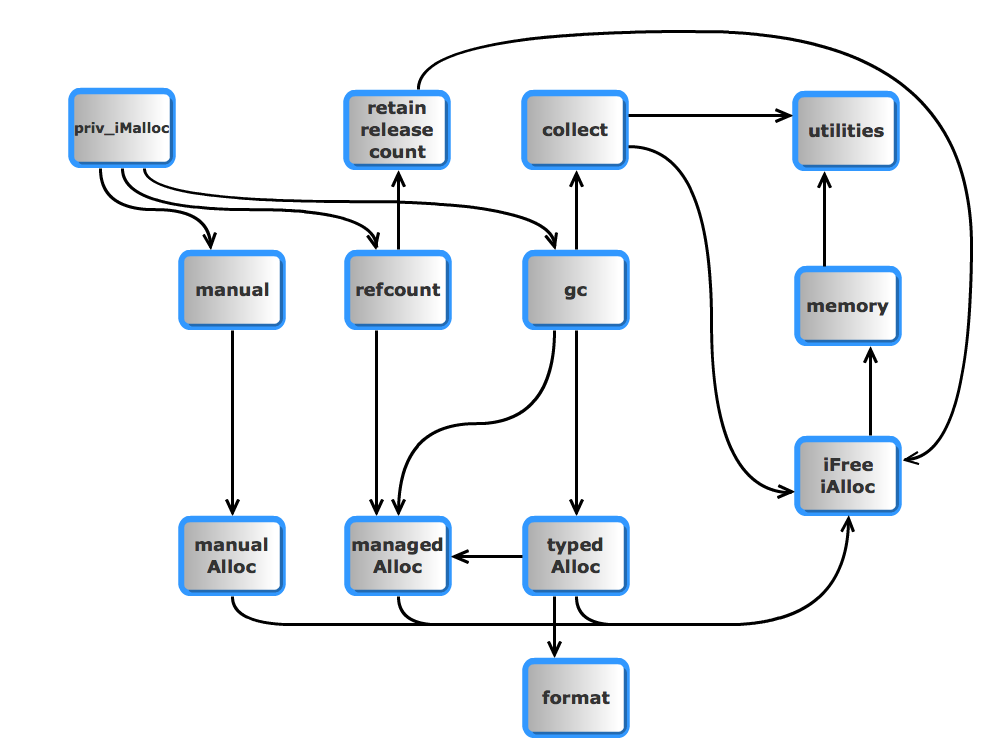
\includegraphics[width=\columnwidth]{../bilder/design_depth.png}
  \caption{En mer djupgående beskrivning av vår design.}
  \label{fig:stable}
\end{figure}





\end{document}

